\documentclass{article}

\usepackage[spanish]{babel}
\usepackage[utf8]{inputenc}
\usepackage[font=footnotesize,labelfont=bf]{caption}
\usepackage{float}
\usepackage{graphicx}
\usepackage{listings}
\usepackage{tikz}

\graphicspath{{images/}}

\title{Trabajo Practico 3: BIP}
\author{Perez, Federico\\
        \texttt{perezfederico@unc.edu.ar}
        \and
        Sardoy, Juan Manuel\\
        \texttt{jmsardoy@gmail.com}
        }
\begin{document}

\maketitle
\begin{center}
    
\includegraphics[scale=2]{unc-logo}
\end{center}
\newpage
\section{Descripción del trabajo}

El siguiente trabajo consiste en la implementación práctica de un módulo completamente
funcional del protocolo UART o "Universal Asynchronous Receiver-Transmitter, en un dispositivo FPGA,
en el lenguaje de descripción de hardware Verilog. \\
Como su nombre lo especifica, se trata de un protocolo asíncrono y \textit{full-duplex}
pero de facil uso e implementación dado su simplicidad.\\
La arquitectura completa del trabajo de aplicación será aproximadamente en siguiente:

\begin{figure}[H]
    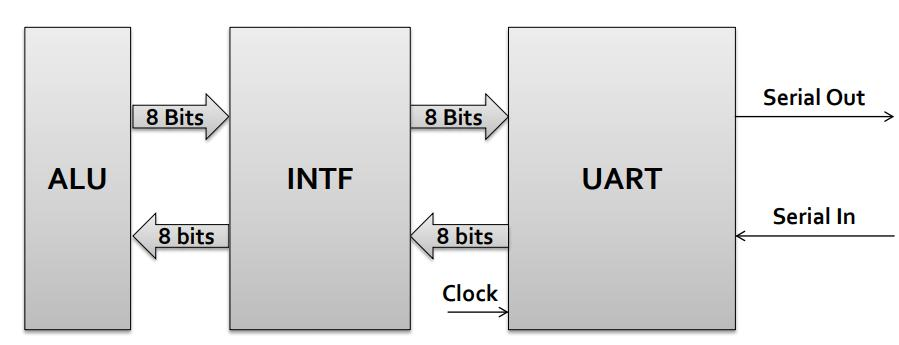
\includegraphics[scale=0.5]{arch}
    \caption{\textit{Diagrama de la arquitectura básica del proyecto}}
\end{figure}

\indent A fines prácticos y demostrativos, dicho módulo UART se conectará mediante un
módulo que actuará de interfaz, a una \textit{Unidad Aritmetico Lógica} o ALU.
Dicho módulo interfaz contendrá lógica que permitirá procesar instrucciones y argumentos recibidos
por el módulo RX del UART, enviarlos a la ALU para su resolución, y reenviarlos por el módulo TX
nuevamente hacia el solicitante del cálculo. \\
\indent Como usuario de dicho sistema, conectaremos el puerto USB de una computadora, y con un convertidor
\textit{USB-UART}, se enviarán las instrucciones y argumentos requeridos. Para dicho fin, además se
desarrollará algún tipo de software que haga uso del hardware convertidor, y facilite el envío de instrucciones
y la recepción de los resultados calculados en la ALU.\\

\newpage
\section{Protocolo UART}
\indent Este protocolo, como se ha explicado anteriormente, es bastante simple. El siguiente diagrama muestra los
datagramas básicos de una comunicación UART.

\begin{figure}[H]
    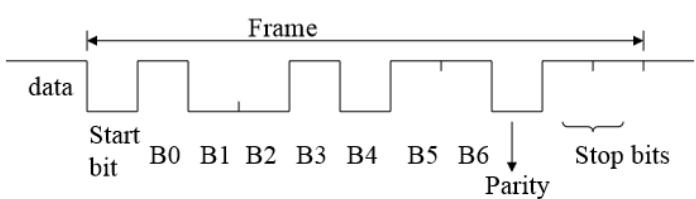
\includegraphics[scale=0.5]{protocol}
    \caption{\textit{Diagrama del datagrama o frame del protocolo UART}}
\end{figure}

\indent El pin RX del receptor, cuando se encuentra en estado de espera o \textit{stand-by}, debe estar en alto o \textit{HIGH}. \\
Cuando se esté por recibir un dato, el nivel baja a \textit{LOW}. Los siguientes siete u ocho bits son de datos, dependiendo si
se utiliza un bit de paridad o no, respectivamente. Luego para finalizar, deben venir dos bits en alto, que indican el final del dato
y se pasa a modo \textit{stand-by} nuevamente. \\
\indent Los dos parámetros mas importantes en una comunicación UART son el \textit{baudrate}, el cual es la frecuencia de símbolos (en este caso \textit{bit}) a la que opera el receptor y transmisor. El otro parametro es si se está usando paridad o no, lo cual afecta la confiabilidad y el tamaño del dato transmitido.

\section{Implementación}
Un transmisor UART es modelado muy facilmente mediante el uso de maquinas de estados finitas (\textit{FSMs o Finite-state machines)},
por esto mismo, se notará que este comportamiento o lógica es replicada en en hardware desarrollado, para ambos modulos RX y TX. \\

\subsection{Generador de Baud Rate}
\indent Dado que un módulo UART puede operar a diferentes \textit{baud rates}, éste debe poseer algun tipo de clock variable que le
sirva como entrada. Básicamente, se trata de un divisor de frecuencia o contador del clock principal. \\
\indent La frecuencia del pulso generado por el generador de baud rate debe ser mayor al baud rate mismo. Esto es para que
el usuario de dicho generador tenga una precición más alta a la hora de leer los bits recibidos. Según estudios ese número es
16 veces, lo que da una ecuación para el contador de la siguiente forma: \\

\begin{figure}[H]
    \begin{center}
        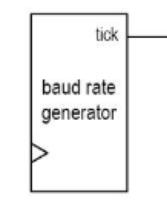
\includegraphics[scale=0.5]{baudrategenerator}
        \caption{\textit{Diagrama del baud-rate generator}}
    \end{center}
\end{figure}

\begin{center}
    $ count = \frac{clock}{baudrate * 16} $
\end{center}

Lo que para un clock de 50Mhz da:

\begin{center}
    $ count = 163 $
\end{center}

Su implementación es la siguiente (ignorando algunas constantes):

\begin{lstlisting}[language=Verilog]
    module BaudRateGenerator
        #(parameter FREQUENCY = `FREQUENCY,
          parameter BAUD_RATE = `BAUD_RATE)
                    (input clk,
                     input rst,
                     output reg out);
-
        localparam MAX_COUNT = (FREQUENCY / (BAUD_RATE * 16));
        localparam COUNT_NBITS = $clog2(MAX_COUNT);

        reg [COUNT_NBITS : 0] count;
        always@(posedge clk or posedge rst)
        begin
            if (!rst) begin
                out <= 0;
                count <= 0;
            end
            else begin
                if(count == MAX_COUNT)
                begin
                    out <= 1;
                    count <= 0;
                end
                else begin
                    out <= 0;
                    count <= count + 1;
                end
            end
        end
    endmodule
\end{lstlisting}

Es simplemente un módulo con dos entradas, el \textit{clock} o \textit{clk} y un pin de \textit{reset} o \textit{rst}, y
un pin de salida o \textit{out}.
Hay un registro \textit{count} que actúa de contador. Dicho contador aumenta con cada ciclo de \textit{clk}.
Cuando el contador llega al valor de \textit{MAX\_COUNT} se invierte el valor de \textit{out}, el cual comienza en 0
luego de un reset.

Vemos como a partir de la frecuencia de operacion, y el \textit{baudrate} elegido,
se calculan el parámetro \textit{MAX\_COUNT}, en tiempo de síntesis.

\subsection{Módulo RX}
\indent El módulo RX o receptor es el encargado de detectar el comienzo de la transmisión por el pin de recepción,
de interpretar los datos, y exponerlo por el bus de salida. Típicamente el bus de salida, y el largo de los datos recibidos
es de un \textit{byte} o 8 \textit{bits}.
\indent Como se podrá notar también a continuación en la implementación del módulo TX, ambos son muy facilmente modelados por máquinas de estado finitas o FSMs dado la naturaleza secuencial de su lógica.
\\
\\
El diagrama de la máquina de estados para el módulo RX es el siguiente:

\begin{figure}[H]
\centering
\begin{tikzpicture}[scale=0.2]
\tikzstyle{every node}+=[inner sep=0pt]
\draw [black] (33.1,-18.5) circle (3);
\draw (33.1,-18.5) node {$IDLE$};
\draw [black] (46.3,-24) circle (3);
\draw (46.3,-24) node {$Start$};
\draw [black] (33.1,-30.6) circle (3);
\draw (33.1,-30.6) node {$Data$};
\draw [black] (20.9,-24.9) circle (3);
\draw (20.9,-24.9) node {$Stop$};
\draw [black] (34.967,-16.18) arc (129.18442:5.57585:7.169);
\fill [black] (46.63,-21.04) -- (47.05,-20.2) -- (46.06,-20.29);
\draw (45.6,-14.57) node [above] {$rx\mbox{ }==\mbox{ }0$};
\draw [black] (46.527,-26.971) arc (-7.07279:-119.79711:7.511);
\fill [black] (35.34,-32.56) -- (35.79,-33.4) -- (36.28,-32.53);
\draw (49.22,-33.3) node [below] {$tick\_count\mbox{ }==\mbox{ }8$};
\draw [black] (31.777,-15.82) arc (234:-54:2.25);
\draw (33.1,-11.25) node [above] {$tx\_start\mbox{ }==\mbox{ }0$};
\fill [black] (34.42,-15.82) -- (35.3,-15.47) -- (34.49,-14.88);
\draw [black] (48.98,-22.677) arc (144:-144:2.25);
\draw (53.55,-24) node [right] {$tick\_count\mbox{ }<\mbox{ }8$};
\fill [black] (48.98,-25.32) -- (49.33,-26.2) -- (49.92,-25.39);
\draw [black] (17.95,-25.376) arc (306.89727:18.89727:2.25);
\draw (13.68,-22.29) node [left] {$tick\_count\mbox{ }<\mbox{ }16$};
\fill [black] (18.73,-22.85) -- (18.65,-21.91) -- (17.85,-22.51);
\draw [black] (31.189,-32.88) arc (-52.71999:-177.36521:6.738);
\fill [black] (20.38,-27.83) -- (19.91,-28.65) -- (20.91,-28.61);
\draw (17.35,-34.18) node [below] {$data\_count\mbox{ }==\mbox{ }8$};
\draw [black] (19.933,-22.085) arc (-173.48478:-311.1531:6.903);
\fill [black] (31.33,-16.1) -- (31.06,-15.2) -- (30.4,-15.95);
\draw (16.28,-14.67) node [above] {$tick\_count\mbox{ }==\mbox{ }16$};
\draw [black] (34.423,-33.28) arc (54:-234:2.25);
\draw (33.1,-37.85) node [below] {$data\mbox{ }<\mbox{ }8$};
\fill [black] (31.78,-33.28) -- (30.9,-33.63) -- (31.71,-34.22);
\end{tikzpicture}
\caption{\textit{Diagrama de estados del módulo RX}}
\end{figure}

La implementación en código es la siguiente:

\begin{lstlisting}[language=Verilog]
module RX(
    input clk,
    input rst,
    input i_baud_rate,
    input i_rx,
    output reg o_rx_done,
    output reg [`NBITS-1 : 0] o_data
);

    localparam NBITS = `NBITS;
    localparam COUNTER_NBITS = $clog2(NBITS)+1;

    localparam
        idle  = 'b00,
        start = 'b01,
        data  = 'b11,
        stop  = 'b10;

    reg [1:0] state, next_state;
    reg [3:0] tick_count, next_tick_count;
    reg [COUNTER_NBITS-1:0] data_count, next_data_count;
    reg [NBITS-1 : 0] next_data;
    reg next_rx_done;

    always@(posedge clk or posedge rst) begin
        if (!rst) begin
            state <= idle;
            tick_count <= 0;
            data_count <= 0;
            o_data <= {NBITS{1'b0}};
            o_rx_done <= 0;
        end
        else begin
            state <= next_state;
            tick_count <= next_tick_count;
            data_count <= next_data_count;
            o_data <= next_data;
            o_rx_done <= next_rx_done;
        end
    end

    always@* begin

        //defaults
        next_state = state;
        next_tick_count = tick_count;
        next_data_count = data_count;
        next_data = o_data;
        next_rx_done = 0;

        case (state)
            idle:
            begin
                if (!i_rx) begin
                    next_state = start;
                    next_tick_count = 0;
                    next_data_count = {COUNTER_NBITS{1'b0}};
                    next_data = {NBITS{1'b0}};
                end
            end
            start:
            begin
                if (i_baud_rate) begin
                    if(tick_count == 7) begin
                        next_state = data;
                        next_tick_count = 0;
                    end
                    else next_tick_count = tick_count + 1;
                end
            end
            data:
            begin
                if (i_baud_rate) begin
                    if (data_count == NBITS) next_state = stop;
                    else begin
                        if(tick_count == 15) begin
                            next_data = {i_rx, o_data[NBITS-1:1]};
                            next_data_count = data_count + 1;
                            next_tick_count = 0;
                        end
                        else next_tick_count = tick_count + 1;
                    end
                end
            end
            stop:
            begin
                if (i_baud_rate) begin
                    if (tick_count == 15) begin
                            next_state = idle;
                            next_rx_done = 1;
                        end
                    else next_tick_count = tick_count + 1;
                end
            end
        endcase
    end
endmodule
\end{lstlisting}

La entradas del módulo son el \textit{clock}, el pin de \textit{reset}, el input del baud rate generator, y el propio pin de comunicaciones o pin \textit{rx}.
A la salida un pin \textit{rx\_done}, que se ocupa de avisar al módulo usuario cuando se recibió un dato, y el bus del dato propiamente recibido.
\indent En cuanto a la implementación, vemos que es la típica de una maquina de estados en Verilog, basada en el diagrama de estados presentado anteriormente.

\subsection{Módulo TX}

El módulo TX del UART es muy similar al RX. Tambien se modela mediante una máquina de estados, la cual es de extrema similitud
con la anteriormente explicada.
\\
\\
Su diagrama de estados es el siguiente:

\begin{figure}[H]
\centering
\begin{tikzpicture}[scale=0.2]
\tikzstyle{every node}+=[inner sep=0pt]
\draw [black] (33.1,-18.4) circle (3);
\draw (33.1,-18.4) node {$Idle$};
\draw [black] (46.3,-24) circle (3);
\draw (46.3,-24) node {$Start$};
\draw [black] (33.1,-30.5) circle (3);
\draw (33.1,-30.5) node {$Data$};
\draw [black] (20.9,-24.8) circle (3);
\draw (20.9,-24.8) node {$Stop$};
\draw [black] (34.986,-16.095) arc (128.74566:5.27691:7.19);
\fill [black] (46.65,-21.04) -- (47.07,-20.2) -- (46.07,-20.29);
\draw (47.75,-14.51) node [above] {$tx\_start\mbox{ }==\mbox{ }1$};
\draw [black] (46.718,-26.95) arc (-3.54174:-124.02475:7.405);
\fill [black] (35.18,-32.63) -- (35.57,-33.49) -- (36.13,-32.66);
\draw (49.87,-33.67) node [below] {$tick\_count\mbox{ }==\mbox{ }16$};
\draw [black] (31.777,-15.72) arc (234:-54:2.25);
\draw (33.1,-11.15) node [above] {$tx\_start\mbox{ }==\mbox{ }0$};
\fill [black] (34.42,-15.72) -- (35.3,-15.37) -- (34.49,-14.78);
\draw [black] (48.98,-22.677) arc (144:-144:2.25);
\draw (53.55,-24) node [right] {$tick\_count\mbox{ }<\mbox{ }16$};
\fill [black] (48.98,-25.32) -- (49.33,-26.2) -- (49.92,-25.39);
\draw [black] (17.95,-25.276) arc (306.89727:18.89727:2.25);
\draw (13.68,-22.19) node [left] {$tick\_count\mbox{ }<\mbox{ }16$};
\fill [black] (18.73,-22.75) -- (18.65,-21.81) -- (17.85,-22.41);
\draw [black] (31.229,-32.813) arc (-51.73413:-178.35107:6.734);
\fill [black] (20.33,-27.72) -- (19.85,-28.53) -- (20.85,-28.5);
\draw (17.3,-34.18) node [below] {$data\_count\mbox{ }==\mbox{ }8$};
\draw [black] (20.046,-21.949) arc (-175.79157:-308.84631:6.891);
\fill [black] (31.24,-16.08) -- (30.93,-15.19) -- (30.3,-15.96);
\draw (16.41,-14.82) node [above] {$tick\_count\mbox{ }==\mbox{ }16$};
\draw [black] (34.423,-33.18) arc (54:-234:2.25);
\draw (33.1,-37.75) node [below] {$data\mbox{ }<\mbox{ }8$};
\fill [black] (31.78,-33.18) -- (30.9,-33.53) -- (31.71,-34.12);
\end{tikzpicture}
\caption{\textit{Diagrama de estados del módulo TX}}
\end{figure}

Su implementación en Verilog es la siguiente:

\begin{lstlisting}[language=Verilog]
module TX(
    input clk,
    input rst,
    input i_baud_rate,
    input i_tx_start,
    input [`NBITS-1 : 0] i_data,
    output reg o_tx_done,
    output reg o_tx);

    localparam NBITS = `NBITS;
    localparam COUNTER_NBITS = $clog2(NBITS)+1;

    localparam
        idle  = 'b00,
        start = 'b01,
        data  = 'b11,
        stop  = 'b10;

    reg [1:0] state, next_state;
    reg [3:0] tick_count, next_tick_count;
    reg [COUNTER_NBITS-1 : 0] data_count, next_data_count;
    reg [NBITS - 1 : 0] data_reg, next_data_reg;
    reg next_tx, next_tx_done;

    always@(posedge clk or posedge rst) begin
        if (!rst) begin
            state <= idle;
            tick_count <= 0;
            data_count <= 0;
            data_reg <= 0;
            o_tx_done <= 1;
            o_tx <= 1;
        end
        else begin
            state <= next_state;
            tick_count <= next_tick_count;
            data_count <= next_data_count;
            data_reg <= next_data_reg;
            o_tx_done <= next_tx_done;
            o_tx <= next_tx;
        end
    end

    always@* begin

        next_tx = o_tx;
        next_tx_done = o_tx_done;
        next_state = state;
        next_tick_count = tick_count;
        next_data_count = data_count;
        next_data_reg = data_reg;

        case (state)
            idle:
            begin
                next_tx = 1;
                next_tx_done = 1;
                if(i_tx_start) begin
                    next_state = start;
                    next_tick_count = 0;
                    next_data_count = 0;
                    next_data_reg = i_data;
                end
            end
            start:
            begin
                next_tx = 0;
                next_tx_done = 0;
                if (i_baud_rate) begin
                    if(tick_count == 15) begin
                        next_tick_count = 0;
                        next_state = data;
                    end
                    else next_tick_count = tick_count + 1;
                end
            end
            data:
            begin
                if (i_baud_rate) begin
                    if (data_count == NBITS) next_state = stop;
                    else begin
                        if(tick_count == 0) begin
                            next_tx = data_reg[0];
                            next_data_reg = data_reg >> 1;
                        end
                        if (tick_count == 15) begin
                            next_tick_count = 0;
                            next_data_count = data_count + 1;
                        end
                        else next_tick_count = tick_count + 1;
                    end
                end
            end
            stop:
            begin
                next_tx = 1;
                if (i_baud_rate) begin
                    if(tick_count == 15) begin
                        next_state = idle;
                    end
                    else next_tick_count = tick_count + 1;
                end
            end
        endcase
    end
endmodule
\end{lstlisting}

En este caso, las entradas al módulo son similares al módulo RX pero en sentido inverso. \textit{clock}, \textit{baudrate} y \textit{reset} se mantienen, pero ahora el bus de datos es la entrada llamado \textit{i\_data}, un pin que indica el momento en el que se debe empezar a enviar datos, llamado \textit{i\_tx\_start}, y de salida, \textit{o\_tx\_done} que indica la finalización del envio, y \textit{o\_tx} que es el pin de la propia comunicación.

\subsection{Módulo Interface}

El módulo interface tiene la utilidad de conectar y controlar el módulo UART con una ALU diseñada en el trabajo práctico
anterior. Lo que hará, sera simplemente esperar dos datos por RX, A y B, y luego un código de operación, realizar la operación solicitada
y enviar el resultado por TX. El usuario de dicho sístema será una computadora, corriendo un script de python, que enviaŕa las operaciones solicitadas y esperará el resultado.

El diagrama de estados del modulo interface es el siguiente:
\\
\\

\begin{figure}[H]
\begin{tikzpicture}[scale=0.2]
\tikzstyle{every node}+=[inner sep=0pt]
\draw [black] (38.7,-15.1) circle (3);
\draw (38.7,-15.1) node {$get\_A$};
\draw [black] (54.8,-22.6) circle (3);
\draw (54.8,-22.6) node {$get\_B$};
\draw [black] (52.2,-40.3) circle (3);
\draw (52.2,-40.3) node {$get\_Opcode$};
\draw [black] (28.7,-38.9) circle (3);
\draw (28.7,-38.9) node {$latch\_result$};
\draw [black] (25.4,-23.5) circle (3);
\draw (25.4,-23.5) node {$send$};
\draw [black] (26.158,-20.609) arc (156.7402:87.81108:10.038);
\fill [black] (35.76,-14.54) -- (34.98,-14.01) -- (34.95,-15.01);
\draw [black] (41.44,-13.904) arc (105.49403:24.55014:10.633);
\fill [black] (53.95,-19.73) -- (54.07,-18.8) -- (53.17,-19.21);
\draw (54.58,-13.97) node [above] {$rx\_done\mbox{ }==\mbox{ }1$};
\draw [black] (56.896,-24.731) arc (36.09399:-52.80713:10.197);
\fill [black] (54.82,-38.86) -- (55.76,-38.78) -- (55.16,-37.98);
\draw (59.44,-32.4) node [right] {$rx\_done\mbox{ }==\mbox{ }1$};
\draw [black] (50.352,-42.655) arc (-44.55028:-142.26839:13.366);
\fill [black] (30.26,-41.46) -- (30.35,-42.4) -- (31.14,-41.78);
\draw (39.61,-47.45) node [below] {$rx\_done\mbox{ }==\mbox{ }1$};
\draw [black] (25.935,-37.776) arc (-122.07248:-213.73801:8.638);
\fill [black] (23.34,-25.66) -- (22.48,-26.05) -- (23.31,-26.6);
\draw [black] (36.663,-12.913) arc (250.69924:-37.30076:2.25);
\draw (31.82,-7.84) node [above] {$rx\_done\mbox{ }==\mbox{ }0$};
\fill [black] (39.2,-12.15) -- (39.93,-11.56) -- (38.99,-11.23);
\draw [black] (57.15,-20.754) arc (155.88866:-132.11134:2.25);
\draw (62.15,-20.87) node [right] {$rx\_done\mbox{ }==\mbox{ }0$};
\fill [black] (57.69,-23.34) -- (58.22,-24.13) -- (58.63,-23.21);
\draw [black] (55.097,-41.032) arc (103.55642:-184.44358:2.25);
\draw (57.89,-46.12) node [right] {$rx\_done\mbox{ }==\mbox{ }0$};
\fill [black] (53.38,-43.04) -- (53.08,-43.94) -- (54.06,-43.71);
\end{tikzpicture}
\caption{\textit{Diagrama de estados del módulo interface}}
\end{figure}

El código Verilog de dicho módulo es:

\begin{lstlisting}[language=Verilog]
module Interface(
    input clk,
    input rst,
    input i_tx_done,
    input i_rx_done,
    input [7:0] i_rx,
    input [7:0] i_alu_result,
    output reg o_tx_start,
    output reg [7:0] o_tx,
    output reg [7:0] o_alu_a,
    output reg [7:0] o_alu_b,
    output reg [5:0] o_alu_opcode,
    output reg [3:0] o_led
);

    localparam
        get_a        = 'b000,
        get_b        = 'b001,
        get_opcode   = 'b010,
        latch_result = 'b011,
        send_result  = 'b100;

    reg [2:0] state, next_state;
    reg next_tx_start;
    reg [7:0] next_tx;
    reg [7:0] next_alu_a;
    reg [7:0] next_alu_b;
    reg [5:0] next_alu_opcode;

    always@(posedge clk or negedge rst) begin
        if(!rst) begin
            state <= get_a;
            o_tx_start <= 0;
            o_tx <= 0;
            o_alu_a <= 0;
            o_alu_b <= 0;
            o_alu_opcode <= 0;
            o_led <= 0;
        end
        else begin
            o_led <= state;
            state <= next_state;
            o_tx_start <= next_tx_start;
            o_tx <= next_tx;
            o_alu_a <= next_alu_a;
            o_alu_b <= next_alu_b;
            o_alu_opcode <= next_alu_opcode;
        end
    end

    always@* begin

        //defaults
        next_state = state;
        next_tx_start = 0;
        next_tx = o_tx;
        next_alu_a = o_alu_a;
        next_alu_b = o_alu_b;
        next_alu_opcode = o_alu_opcode;

        case (state)
            get_a:
            begin
                if(i_rx_done) begin
                    next_alu_a = i_rx;
                    next_state = get_b;
                end
            end
            get_b:
            begin
                if(i_rx_done) begin
                    next_alu_b = i_rx;
                    next_state = get_opcode;
                end
            end
            get_opcode:
            begin
                if(i_rx_done) begin
                    next_alu_opcode = i_rx[5:0];
                    next_state = latch_result;
                end
            end
            latch_result:
            begin
                next_tx = i_alu_result;
                next_state = send_result;
            end
            send_result:
            begin
                next_tx_start = 1;
                next_state = get_a;
            end
        endcase
    end
endmodule
\end{lstlisting}

\subsection{Aplicación}

Una vez implementado prácticamente el módulo UART, se procedió comprobar su funcionamiento mediante la medición
del voltaje del pin de salida \textit{TX} con un osciloscopio durante el funcionamiento de este.
A modo de ejemplo de una de las lecturas, se incluye una imagen demostrativa de la pantalla de instrumento
en dicha medición:

\begin{figure}[H]
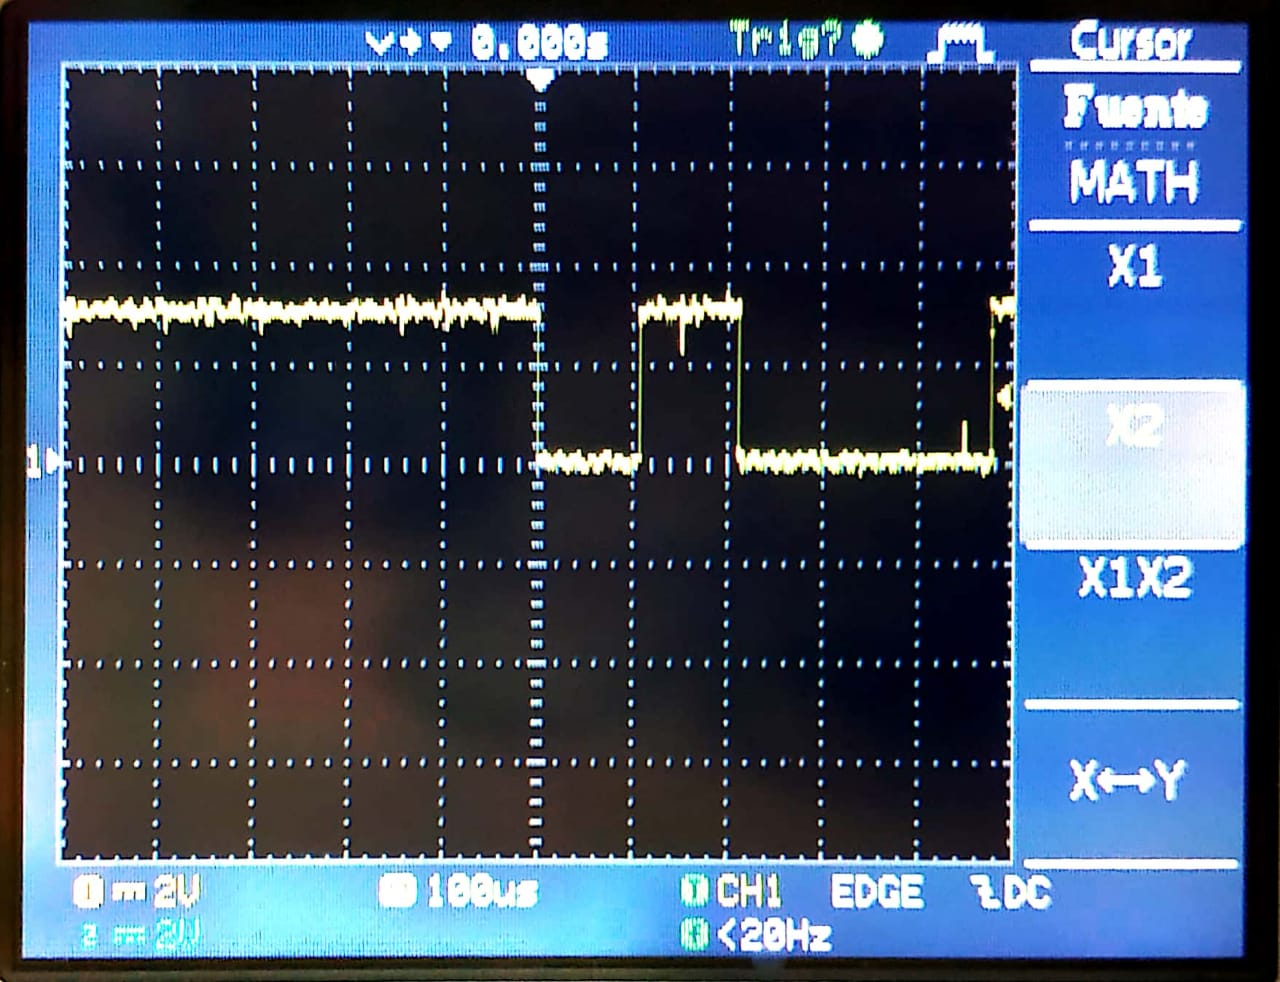
\includegraphics[scale=0.25]{osc}
\caption{\textit{Lectura del osciloscopio al enviar un dato por TX}}
\end{figure}

\end{document}
